\section{The figures}
\label{sec:figures}

\Cref{tab:params} collects the parameter values of every figure. Unless a
figure states otherwise, it uses the baseline of \Cref{sec:model}:
$k = 0.1$, $u_R = 1$, the transition matrix $Q$ above, and the grid of
\Cref{sec:procedure}.

\begin{table}[htbp]
\caption{Parameter values by figure}
\label{tab:params}
\centering
\small
\begin{tabular}{@{}p{3.3cm}p{3.4cm}p{8.6cm}@{}}
\toprule
Figure & Axes & Departure from the baseline \\
\midrule
1.4 & $c \in [0, 5]$, $\delta \in [0, 1]$ & none \\
Main paper, Figure 6 & $c \in [0, 5]$, $\delta \in [0, 1]$ & two-leader variant: fifth state $N$, $5 \times 5$ transition matrix, payoffs at $N$ by action pair, third probability $\lambda_N$ (\Cref{sec:model}) \\
1.5 & same data as 1.4 & white curve $c = f(\delta)$, the planner's threshold (\Cref{sec:fig15}) \\
1.6 & same data as 1.4 & four-class colors and the same white curve \\
1.9 & $\gamma \in [0, 0.1]$, $\delta \in [0, 1]$ & $c = 1.5$; rules payoffs $(1 + \gamma,\, 1 + \gamma,\, 1 - \kappa\gamma,\, 1 - \kappa\gamma)$ at $(\hI, \dI, \dJ, \hJ)$ with $\kappa = 1.5$ \\
1.B.3 & $c \in [0, 5]$, $\delta \in [0, 1]$ & $q_{\dI,\dI} = q_{\dJ,\dJ} = q \in \{0.35, 0.60, 0.85, 0.99\}$, with rows $Q_{\dI} = (\tfrac{1-q}{2}, q, \tfrac{1-q}{2}, 0)$ and $Q_{\dJ} = (0, \tfrac{1-q}{2}, q, \tfrac{1-q}{2})$ \\
1.F.1 & $c \in [0, 5]$, $\delta \in [0, 1]$ & under power, $Q^P_{\dI} = (0.45, 0.10 + \eta, 0.45 - \eta, 0)$ and $Q^P_{\dJ} = (0, 0.45 - \eta, 0.10 + \eta, 0.45)$ with $\eta = \bar\eta = 0.45$; under rules, $Q$ as in the baseline \\
2.1 (P\&P 1) & $q_{0,0} \in [0, 1]$ & multipolar model: $c = 8$, $\delta = 0.4$, $N \in \{3, 6\}$, $\varphi(N) = 1.52\, e^{-0.165 N}$ \\
\bottomrule
\end{tabular}
\end{table}

\subsection{Figure 1.4, Symmetric Markovian equilibria}
\label{sec:fig14}

\code{main\_RPC.m} solves the baseline model on the $(c, \delta)$ grid and
saves \code{main\_2112.mat}; \code{make\_figures.m} draws it with three
classes and no overlay (\Cref{fig:14}).

Three features of the map follow directly from the model. First, the cyclic
region (blue) lies to the left of $c = 1$. Under cyclic play the rules built
at $\hI$ are broken as soon as the world turns bipolar, so the hegemon's
return to building is essentially the static gain $u_R - u^P(\hI) - c =
1 - c$, which is positive only if $c < 1$; the exact boundary is
$c\,(1 - q_{\hI,\hI}\delta) = 1$, within one grid step of the vertical line.
Second, for $c > 1$ building pays only if the rules survive the bipolar
phase, which requires the dominant country to keep them ($\lambda_2 = 1$)
and the hegemon to be patient enough to recoup $c$; the rules-based region
(green) is therefore bounded below by a $\delta$ threshold that rises with
$c$, and the transition is the blurred band of mixed strategies described
in \Cref{sec:procedure}. Third, the boundary between the cyclic and the
rules-based regions for $c < 1$ rises as $c$ falls: when rules are cheap to
rebuild, a dominant country loses little by breaking them, so more patience
is needed to keep them. Everything below these thresholds is power-based
(red).

\begin{figure}[htbp]
\centering
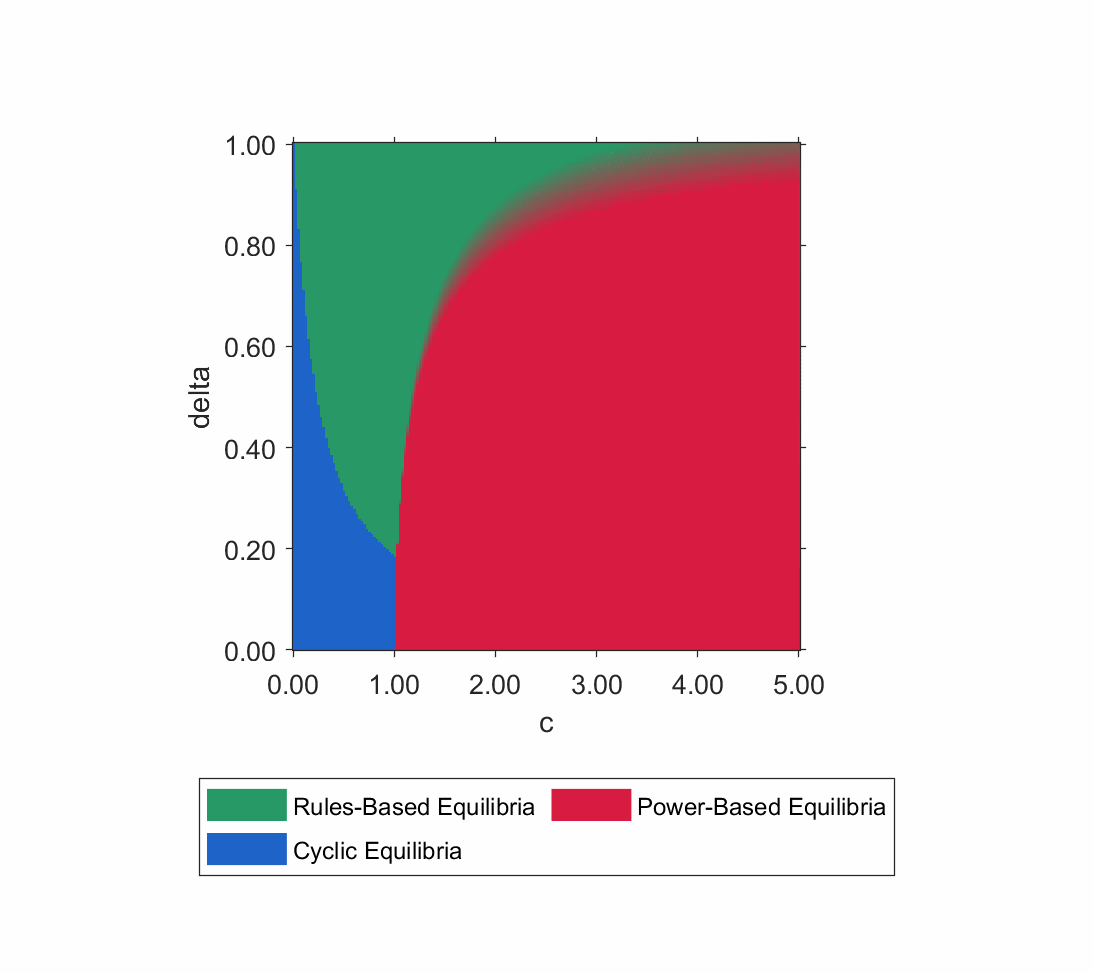
\includegraphics[width=0.62\linewidth]{fig_1_4_symmetric_markovian.png}
\caption{Figure 1.4, Symmetric Markovian equilibria (baseline parameters)}
\label{fig:14}
\begin{minipage}{0.9\linewidth}
\vspace{4pt}
\footnotesize\raggedright
\textit{Notes:} \code{main\_RPC.m} $\rightarrow$ \code{main\_2112.mat}
$\rightarrow$ \code{plot\_map(\ldots, 'plot\_RPC.png', false, false)}.
\end{minipage}
\end{figure}

\subsection{Figure 1.5, Efficient and inefficient equilibria}
\label{sec:fig15}

The figure overlays on the data of Figure 1.4 the locus of building costs at
which a social planner is indifferent between permanent rules and permanent
power (\Cref{fig:15}). Let $W_h$ and $W_d$ denote the joint discounted
payoff of the two countries under permanent power, starting from a
hegemonic and a dominance state. With joint per-period payoffs of $0$ in
hegemonic states and $1.9$ in dominance states, the baseline transitions
give
\begin{align*}
  W_h &= \delta\,(0.1\, W_h + 0.9\, W_d), \qquad
  W_d = 1.9 + \delta\,(0.45\, W_h + 0.55\, W_d),
\end{align*}
so that $W_h = 1.71\,\delta / (1 - 0.65\,\delta - 0.35\,\delta^2)$.
Permanent rules built in a hegemonic state are worth $2/(1 - \delta) - c$,
so building is efficient if and only if $c \leq f(\delta)$, where
\begin{align*}
  f(\delta) = \frac{2}{1 - \delta} - \frac{1.71\,\delta}{1 - 0.65\,\delta - 0.35\,\delta^2}.
\end{align*}
The white curve is $c = f(\delta)$, coded in \code{plot\_map.m} and drawn
when the argument \code{social\_planner} is true; it starts at $c = 2$ for
$\delta = 0$ and grows without bound as $\delta \to 1$. Power-based
equilibria to the left of the curve are inefficient, because a planner would
build rules. Cyclic equilibria are inefficient everywhere, because keeping
rules costs nothing and raises the joint payoff by $k$ in every bipolar
period. The two white labels are written on the PNG by
\code{legend\_merger.py}.

\begin{figure}[htbp]
\centering
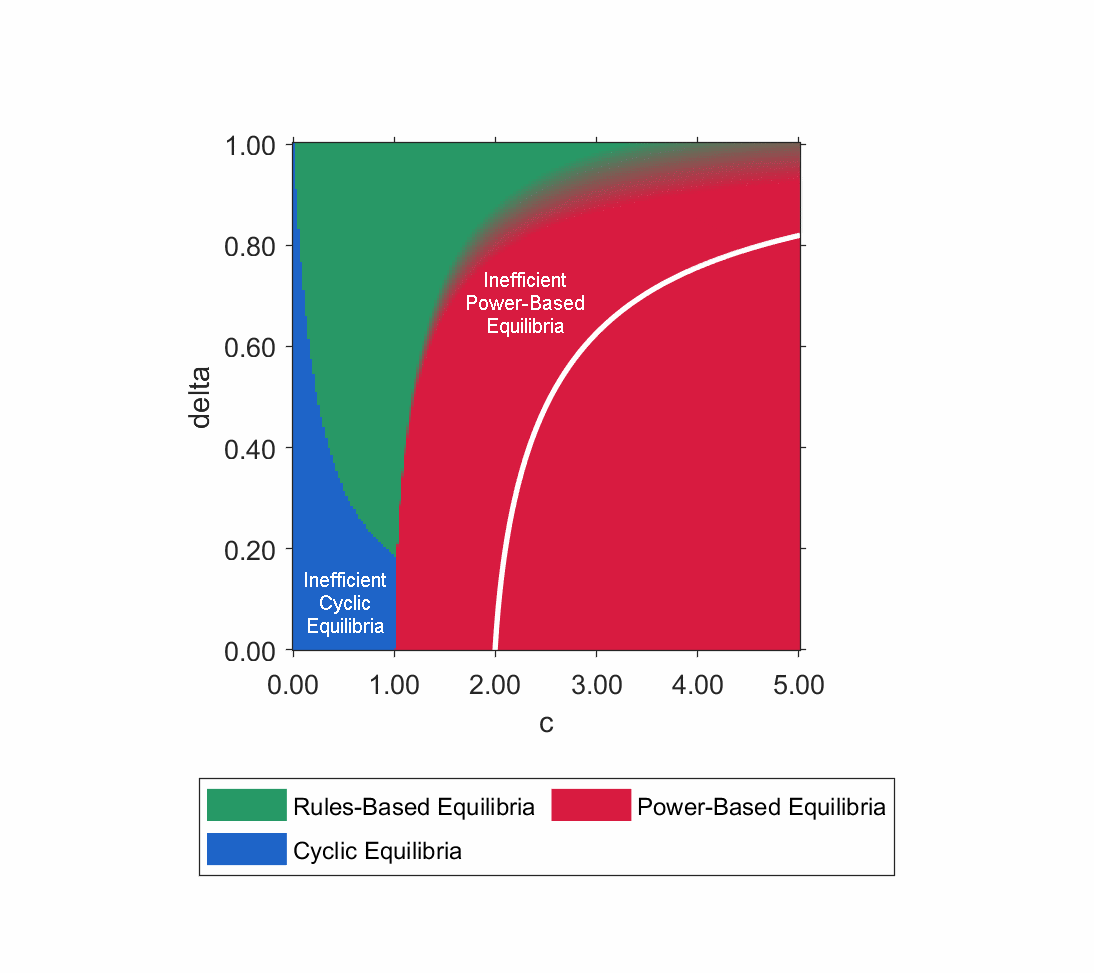
\includegraphics[width=0.62\linewidth]{fig_1_5_efficient_inefficient.png}
\caption{Figure 1.5, Efficient and inefficient equilibria}
\label{fig:15}
\begin{minipage}{0.9\linewidth}
\vspace{4pt}
\footnotesize\raggedright
\textit{Notes:} \code{main\_2112.mat} $\rightarrow$
\code{plot\_map(\ldots, 'plot\_socialPlanner.png', true, false)}
$\rightarrow$ \code{legend\_merger.py}.
\end{minipage}
\end{figure}

\subsection{Figure 1.6, Rules-resistant and rules-compatible power-based equilibria}
\label{sec:fig16}

Same data and same white curve as Figure 1.5, drawn with four classes
(\Cref{fig:16}): the power-based region is split by $\lambda_2$ into
rules-compatible equilibria (orange, the dominant country would keep rules
if they existed) and rules-resistant equilibria (red, it would break them).
Because no rules are built along the path of a power-based equilibrium, $c$
does not enter the dominant country's comparison, and the boundary between
the two classes is horizontal at the $\delta$ at which the static gain from
breaking rules, $k = 0.1$, equals the discounted loss from a bipolar world
without rules (about $\delta = 0.17$ in the baseline). The labels
``Inefficient RCP Equilibria'' and ``Inefficient RRP Equilibria'' are
written by \code{legend\_merger.py}.

\begin{figure}[htbp]
\centering
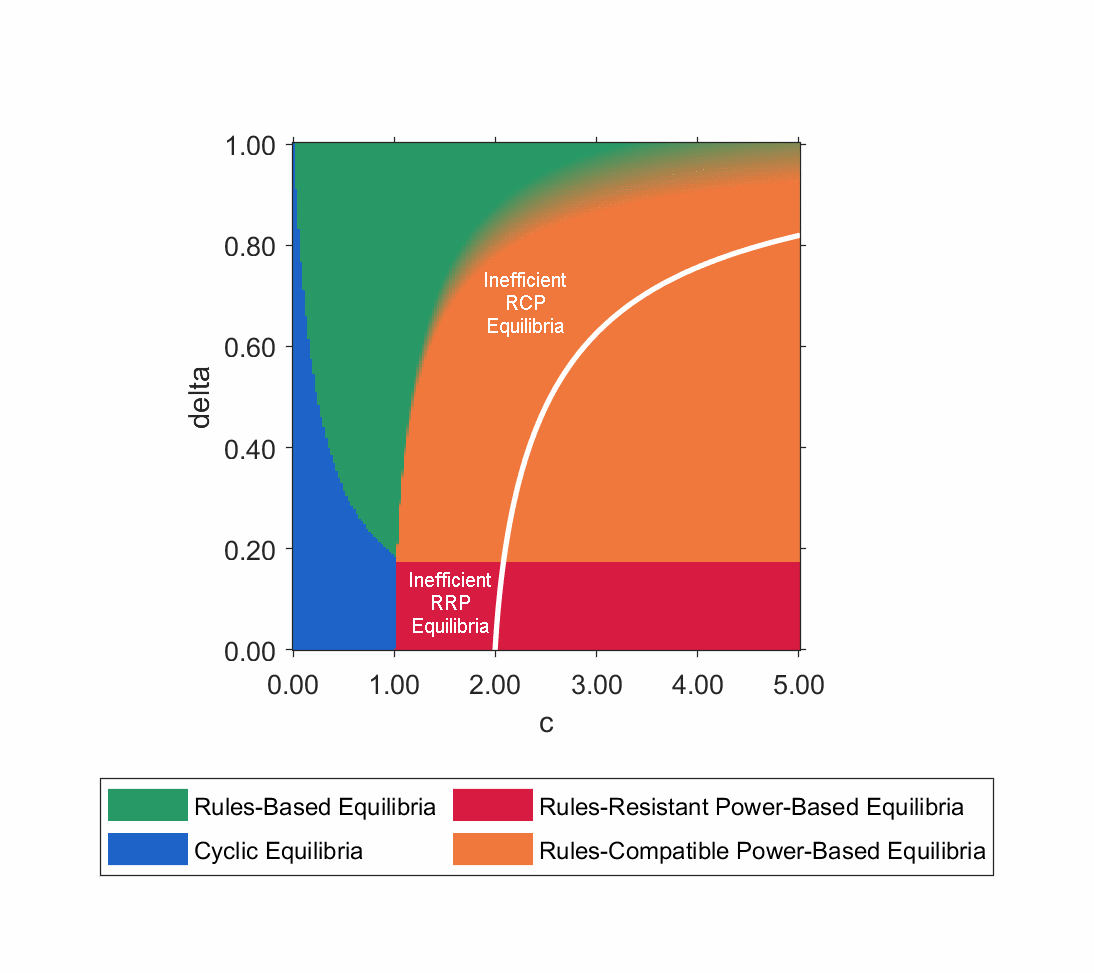
\includegraphics[width=0.62\linewidth]{fig_1_6_rules_resistant_compatible.png}
\caption{Figure 1.6, Rules-resistant and rules-compatible power-based equilibria}
\label{fig:16}
\begin{minipage}{0.9\linewidth}
\vspace{4pt}
\footnotesize\raggedright
\textit{Notes:} \code{main\_2112.mat} $\rightarrow$
\code{plot\_map(\ldots, 'plot\_socialPlanner\_fourClasses.png', true, true)}
$\rightarrow$ \code{legend\_merger.py}.
\end{minipage}
\end{figure}

\subsection{Figure 1.9, Sustainability of a rules-lite regime with $c = 1.5$}
\label{sec:fig19}

\code{main\_uRDelta.m} fixes $c = 1.5$ and replaces the building cost on
the horizontal axis by a tilt $\gamma \in [0, 0.1]$ of the rules in favor of
the leading country (the code calls it \code{l}). Under rules the hegemon
and the dominant country receive $1 + \gamma$, and the follower receives
$1 - \kappa\gamma$ at $\dJ$ and $\hJ$, with $\kappa = 1.5$; payoffs under
power are the baseline ones. With $\kappa > 1$ the tilt is not a pure
transfer: it lowers the joint payoff under rules by $(\kappa - 1)\gamma$ per
period. The script saves \code{main\_kappa15\_c15.mat} (the name encodes
$10\kappa$ and $10c$), and \code{plot\_map\_gamma.m} draws it with four
classes (\Cref{fig:19}). The legend lists three classes because no cyclic
equilibrium exists at $c = 1.5 > 1$.

The rules-resistant region at the bottom shrinks as $\gamma$ grows and
vanishes at $\gamma = k = 0.1$, where the dominant country's static gain
from breaking the rules, $k - \gamma$, reaches zero. The lower boundary of
the rules-based region declines with $\gamma$ because the hegemon's gain
from building rules, $1 + \gamma - c$ per period of hegemony, rises with the
tilt. The other runs of the same script kept in the working folder
($\kappa \in \{1, 2\}$, $c \in \{0.1, 0.5\}$) were explorations and are not
in the paper.

\begin{figure}[htbp]
\centering
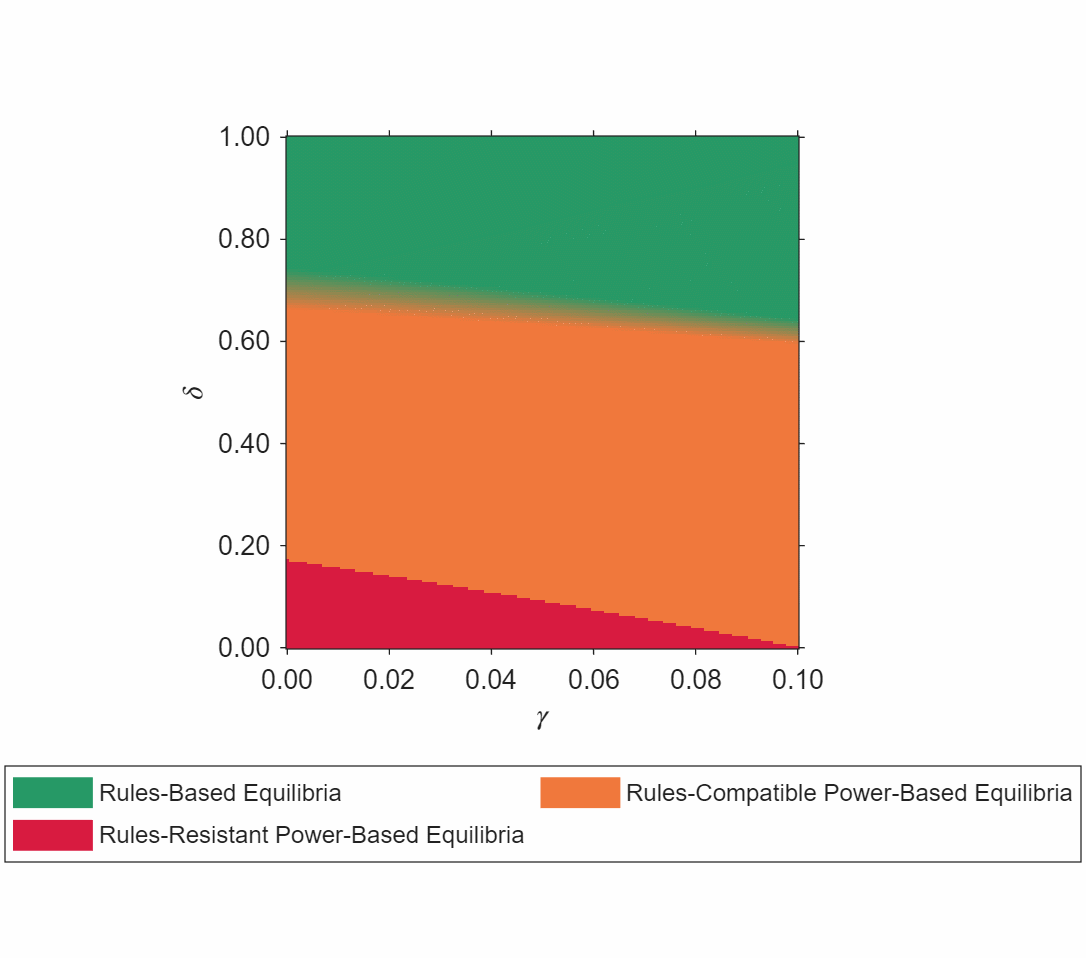
\includegraphics[width=0.62\linewidth]{fig_1_9_rules_lite_c15.png}
\caption{Figure 1.9, Sustainability of a rules-lite regime with $c = 1.5$}
\label{fig:19}
\begin{minipage}{0.9\linewidth}
\vspace{4pt}
\footnotesize\raggedright
\textit{Notes:} \code{main\_uRDelta.m} ($c = 1.5$, $\kappa = 1.5$)
$\rightarrow$ \code{main\_kappa15\_c15.mat} $\rightarrow$
\code{plot\_map\_gamma(\ldots, 'rules\_lite\_c15.png', false, true)}.
\end{minipage}
\end{figure}

\subsection{Figure 1.B.3, Enduring dominance}
\label{sec:fig1B3}

\code{main\_RPC\_changingQ22.m} runs the baseline solver four times, once
for each persistence of the dominance states $q \in \{0.35, 0.60, 0.85,
0.99\}$. It sets $q_{\dI,\dI} = q_{\dJ,\dJ} = q$ and splits the remaining
probability equally between the two neighboring states, so the rows of
$\dI$ and $\dJ$ become $(\tfrac{1-q}{2}, q, \tfrac{1-q}{2}, 0)$ and
$(0, \tfrac{1-q}{2}, q, \tfrac{1-q}{2})$; the hegemonic rows and all payoffs
are the baseline ones. Each run saves \code{prop4\_XX.mat} with $\mathit{XX} = 100q$ (the
script is named after Proposition 4), \code{make\_figures.m} draws the four
three-class maps, and \code{image\_merger.py} crops them, adds the
\LaTeX{} titles $q_{\dI,\dI} = \ldots$, and stacks them with a single
legend (\Cref{fig:1B3}).

As dominance becomes more persistent the rules-based region recedes toward
$\delta = 1$ and the cyclic region grows: a dominant country that expects
to stay dominant for long has little to gain from the rules it would enjoy
as a follower, so it breaks them unless it is very patient. At $q = 0.99$
no rules-based equilibrium remains on the grid; the map shows cyclic
equilibria for $c < 1$ and power-based equilibria otherwise.

\begin{figure}[htbp]
\centering
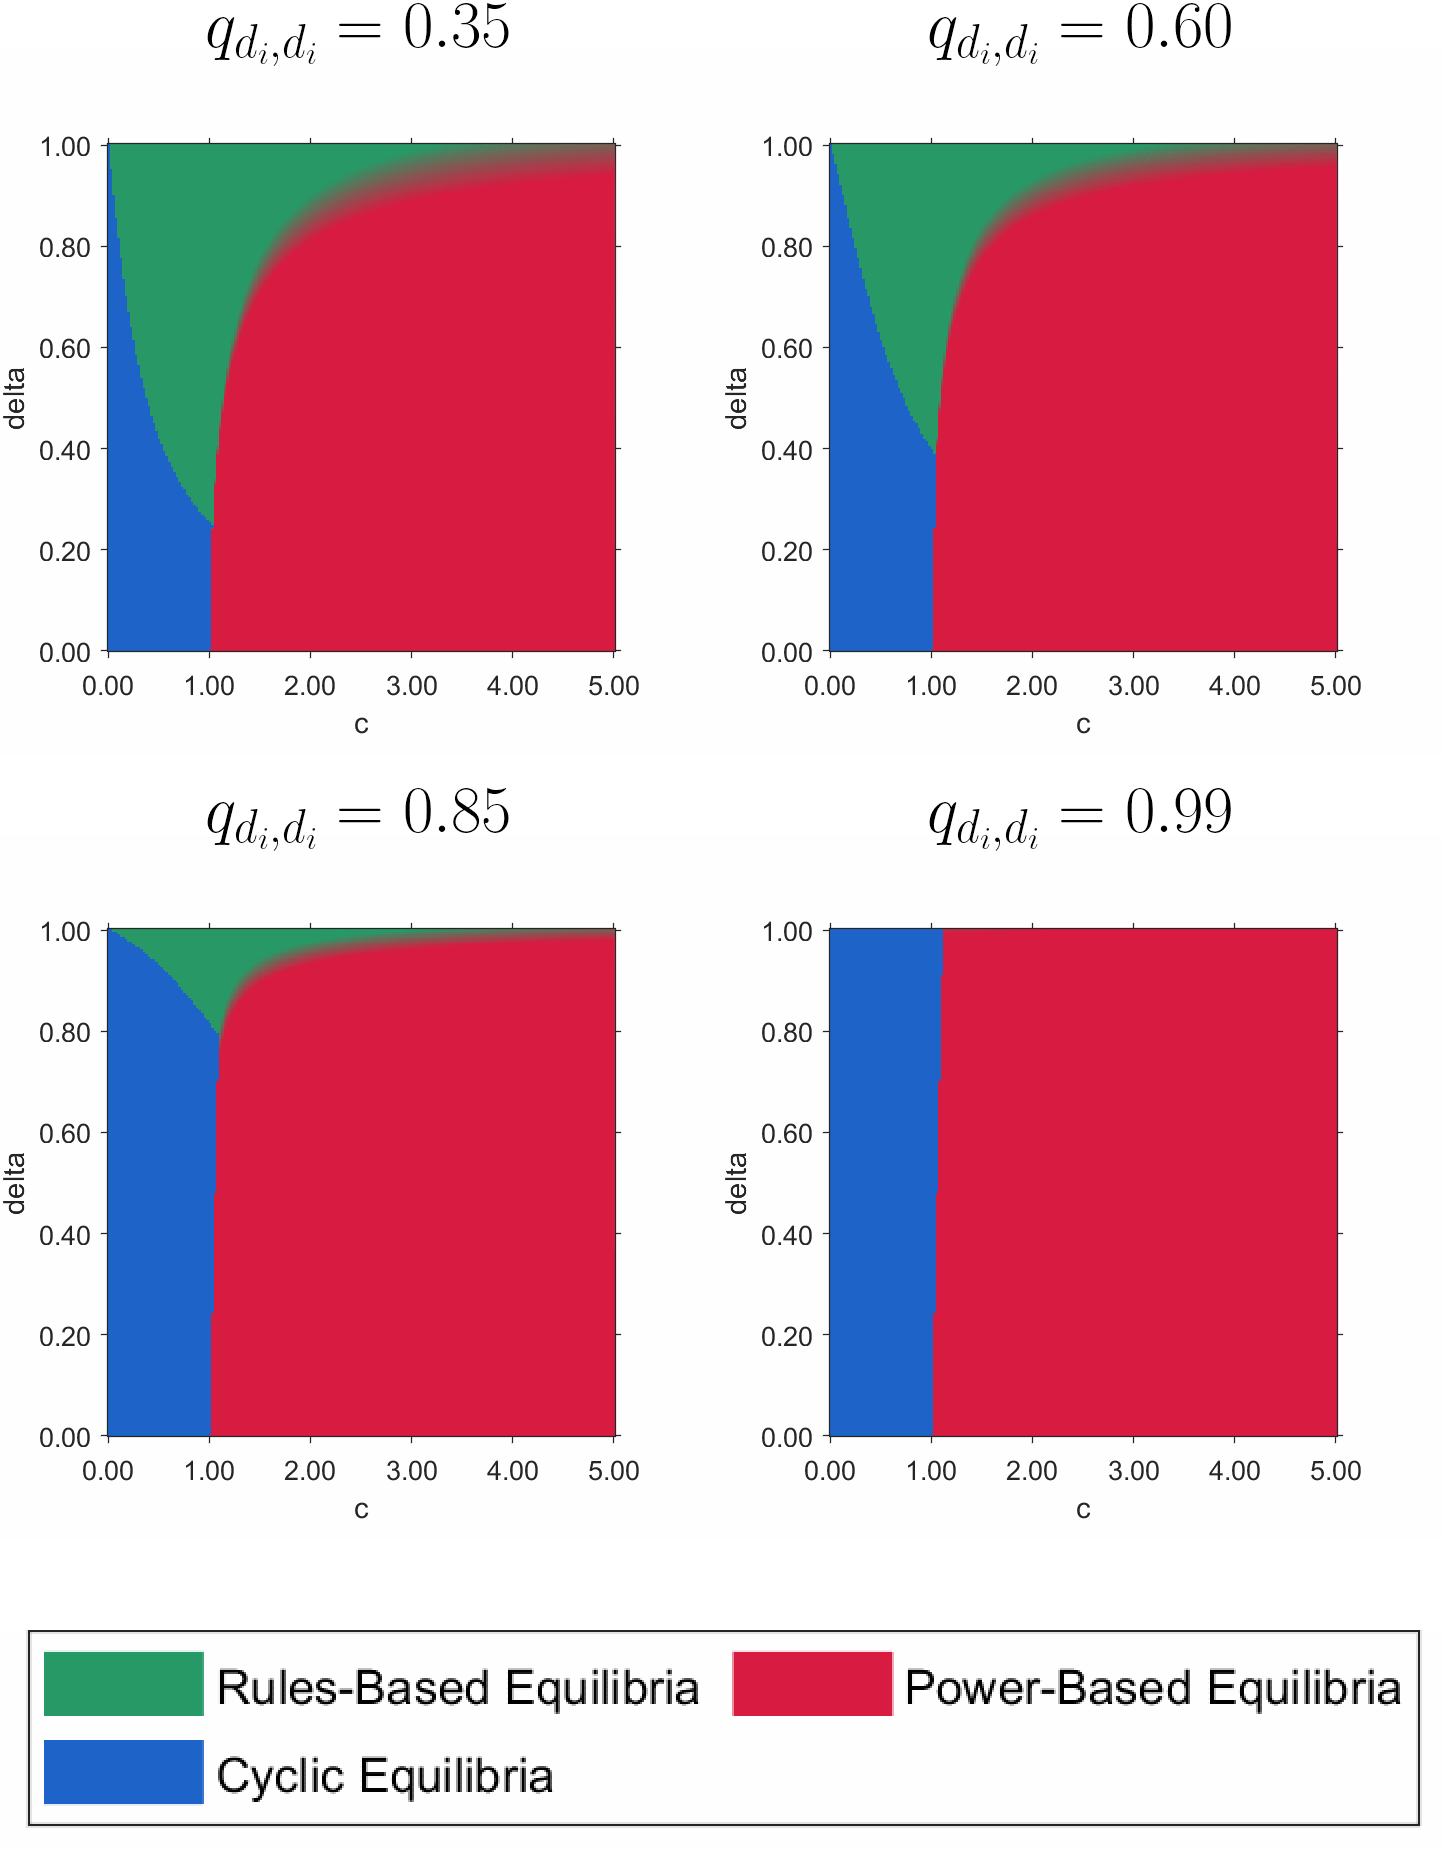
\includegraphics[height=0.55\textheight]{fig_1_B_3_enduring_dominance.png}
\caption{Figure 1.B.3, Enduring dominance}
\label{fig:1B3}
\begin{minipage}{0.9\linewidth}
\vspace{4pt}
\footnotesize\raggedright
\textit{Notes:} \code{main\_RPC\_changingQ22.m} $\rightarrow$
\code{prop4\_\{35,60,85,99\}.mat} $\rightarrow$
\code{plot\_map(\ldots, 'plot\_prop4\_XX.png', false, false)} $\rightarrow$
\code{image\_merger.py}.
\end{minipage}
\end{figure}

\subsection{Figure 1.F.1, Equilibria under endogenous transitions, $\eta = \bar\eta$}
\label{sec:fig1F1}

\code{main\_RPC\_newEndogenous.m} lets the choice of power in a dominance
state raise the chance of remaining dominant. The script's variable
\code{gamma} is the paper's $\eta$: under power, probability mass $\eta$
moves from $q_{\dI,\dJ}$ to $q_{\dI,\dI}$ (and symmetrically at $\dJ$),
so the rows of $\dI$ and $\dJ$ become $(0.45, 0.10 + \eta, 0.45 - \eta, 0)$
and $(0, 0.45 - \eta, 0.10 + \eta, 0.45)$, while under rules the baseline
rows apply. The figure uses $\eta = \bar\eta = 0.45$, the largest shift
that keeps every probability nonnegative, so a dominant country that plays
power never hands its lead to the other country directly. The modified
rows enter every continuation value under power at $\dI$ and $\dJ$,
including the deviation values in conditions (b) and (d). The script saves
\code{endogenous\_2213.mat}, and \code{make\_figures.m} draws it with four
classes and no overlay (\Cref{fig:1F1}).

Compared with Figure 1.6, the rules-resistant region is larger (its upper
boundary moves from about $\delta = 0.17$ to about $0.22$), because power
now also buys persistence of the dominant position. All boundaries are
sharp: the solver found a pure-strategy equilibrium at every grid point of
this run.

\begin{figure}[htbp]
\centering
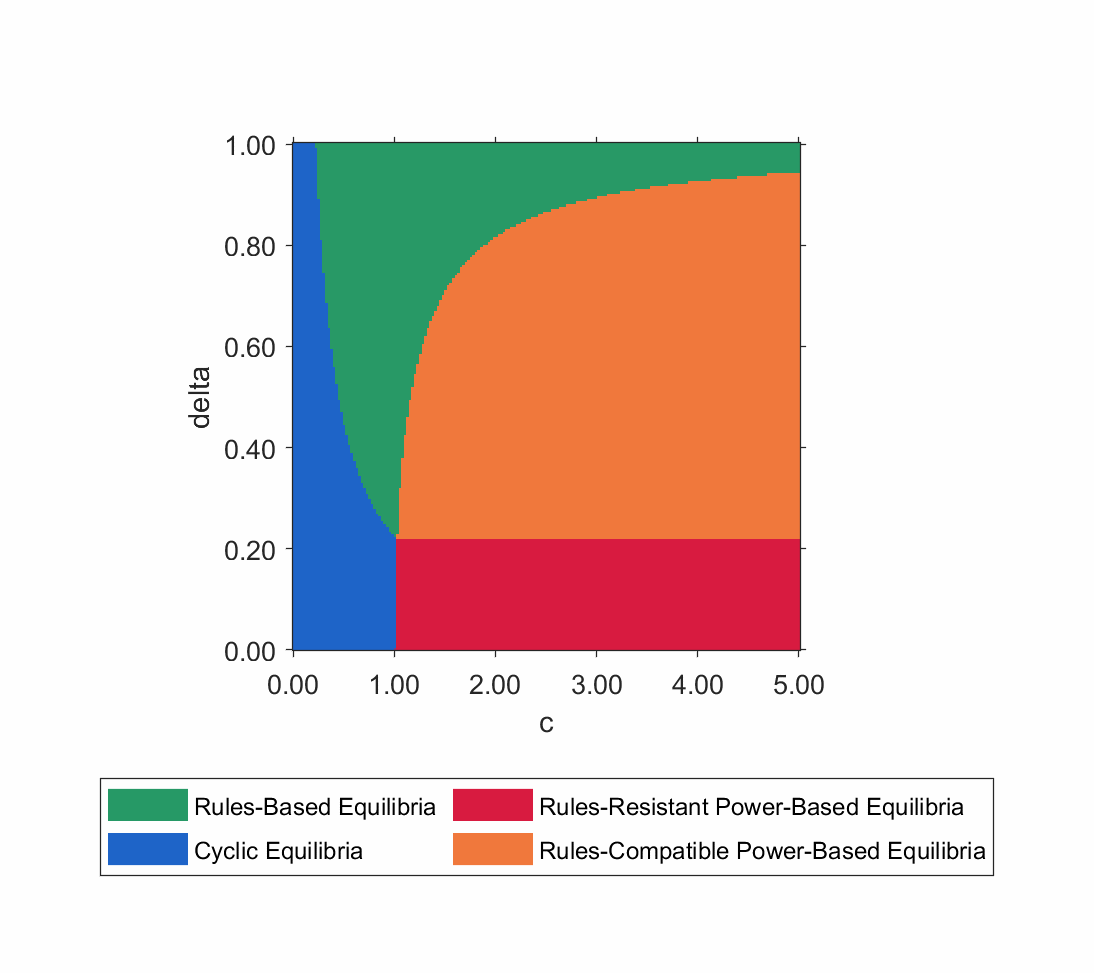
\includegraphics[width=0.62\linewidth]{fig_1_F_1_endogenous_transitions.png}
\caption{Figure 1.F.1, Equilibria under endogenous transitions, $\eta = \bar\eta$}
\label{fig:1F1}
\begin{minipage}{0.9\linewidth}
\vspace{4pt}
\footnotesize\raggedright
\textit{Notes:} \code{main\_RPC\_newEndogenous.m} ($\eta = 0.45$)
$\rightarrow$ \code{endogenous\_2213.mat} $\rightarrow$
\code{plot\_map(\ldots, 'plot\_endogenous.png', false, true)}.
\end{minipage}
\end{figure}

\subsection{Figure 6 of the main paper, Rules-based equilibria in a bipolar world}
\label{sec:fig6}

This figure belongs to the main paper, ``Equilibrium Trade Regimes: Power-
vs. Rules-Based'' (Carvalho, Monte, and Ornelas, CEPR DP 20751).
\code{main\_RPC\_dotProduct\_twoLeader.m} solves the two-leader variant of
\Cref{sec:model} on the same $(c, \delta)$ grid, with $k = 0.1$, $u_R = 1$,
and the five-state transition matrix, and saves
\code{twoLeaders\_1519.mat}, which holds the three strategy matrices.
\code{make\_figures.m} draws it with \code{plot\_map\_twoLeaders.m} as a
three-class map and no overlay (\Cref{fig:6}). The figure looks like
Figure 1.4 but is a different run: rules now also have to survive the
multipolar state, where each leader gains $k$ in the short run from playing
power and the regime collapses unless both refrain. The cyclic region is
therefore larger (it reaches about $\delta = 0.45$ at $c = 1$, against
$0.2$ in Figure 1.4) and the rules-based region starts at higher $\delta$
for every $c$. The solver found mixed strategies in a thinner band than in
the baseline.

\begin{figure}[htbp]
\centering
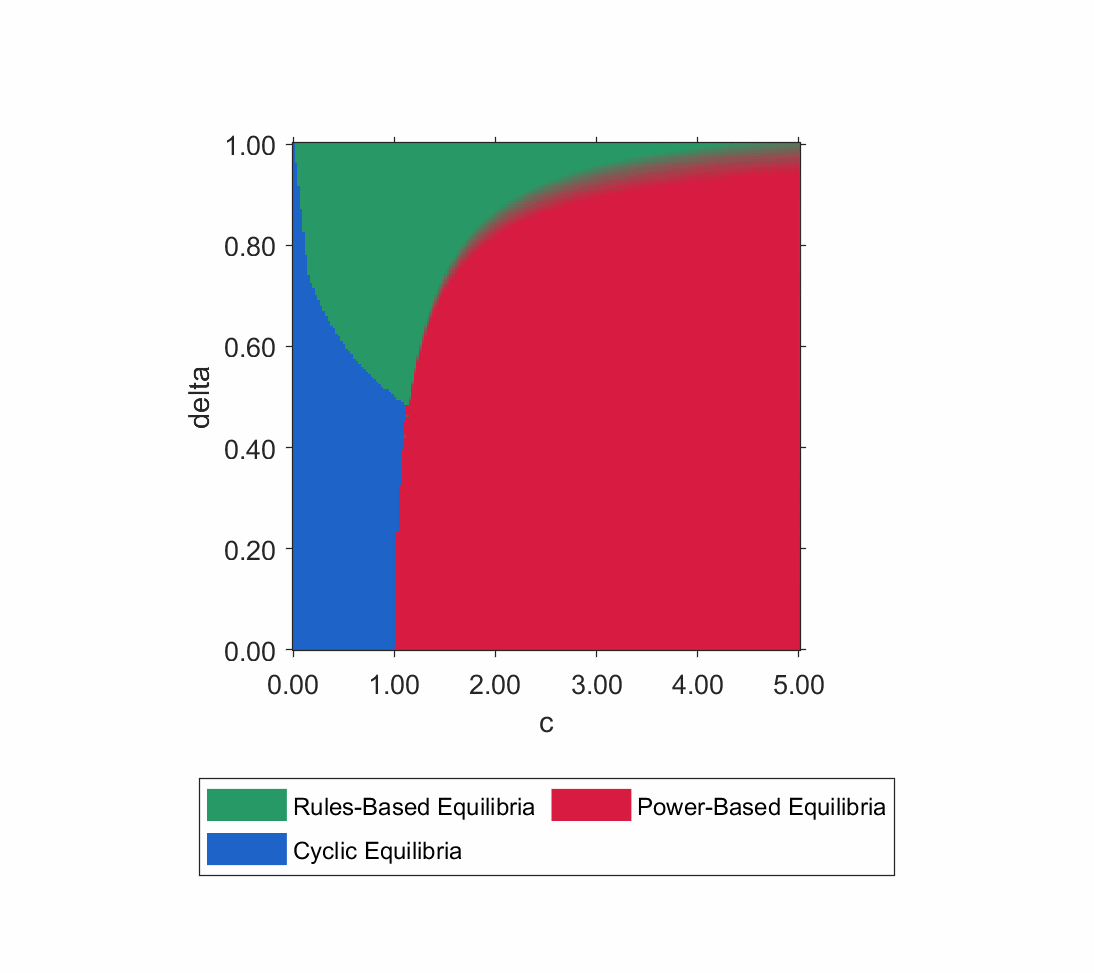
\includegraphics[width=0.62\linewidth]{fig_6_bipolar_world.png}
\caption{Figure 6 of ``Equilibrium Trade Regimes: Power- vs. Rules-Based'', Rules-based equilibria in a bipolar world (two-leader model)}
\label{fig:6}
\begin{minipage}{0.9\linewidth}
\vspace{4pt}
\footnotesize\raggedright
\textit{Notes:} \code{main\_RPC\_dotProduct\_twoLeader.m} $\rightarrow$
\code{twoLeaders\_1519.mat} $\rightarrow$
\code{plot\_map\_twoLeaders(\ldots, 'plot\_twoLeaders\_three.png', false, false)}.
\end{minipage}
\end{figure}

\subsection{Figure 2.1, Multipolar fragmentation and persistence (P\&P Figure 1)}
\label{sec:fig21}

This figure belongs to the multipolar model of the P\&P paper. The Python
script \code{persistence.py} produces it without any solver. With symmetric
transitions out of the multipolar state, so that $q_{0,i} = (1 - q_{0,0})/N$
for every country $i$, the paper's sustainability condition for rules
compares a dynamic benefit with a static cost. The script plots, as
functions of the multipolar persistence $x = q_{0,0} \in [0, 1]$,
\begin{align*}
  \text{efficiency advantage} &= \frac{\delta x}{1 - \delta x}, \\
  \text{hegemony prospects} &= \frac{c\,\delta}{N}\,\frac{1 - x}{1 - \delta x}, \\
  \text{total benefit} &= \text{efficiency advantage} + \text{hegemony prospects}, \\
  \text{total cost} &= \varphi(N) = 1.52\, e^{-0.165 N},
\end{align*}
with $c = 8$, $\delta = 0.4$, and one panel for each $N \in \{3, 6\}$. The
cost $\varphi(N)$ is the one-shot deviation gain under the payoff
specification of the paper's footnote, where multipolar payoffs are
$2 n_i/(N - 1) - 1$ under rules and $(n_i/(N - 1))(1 + \varphi(N))$ under
power, $n_i$ being the number of other countries choosing rules. The bar
along the horizontal axis is green where the total benefit exceeds the cost
(a rules-based equilibrium coexists with the cyclic one) and blue where it
does not (only the cyclic equilibrium exists). The script writes
\code{persistence.pdf}, which the P\&P manuscript includes as
\code{Figure1.pdf} (\Cref{fig:21}); the colors are the green and blue of
the maps and the font is Times New Roman.

\begin{figure}[htbp]
\centering
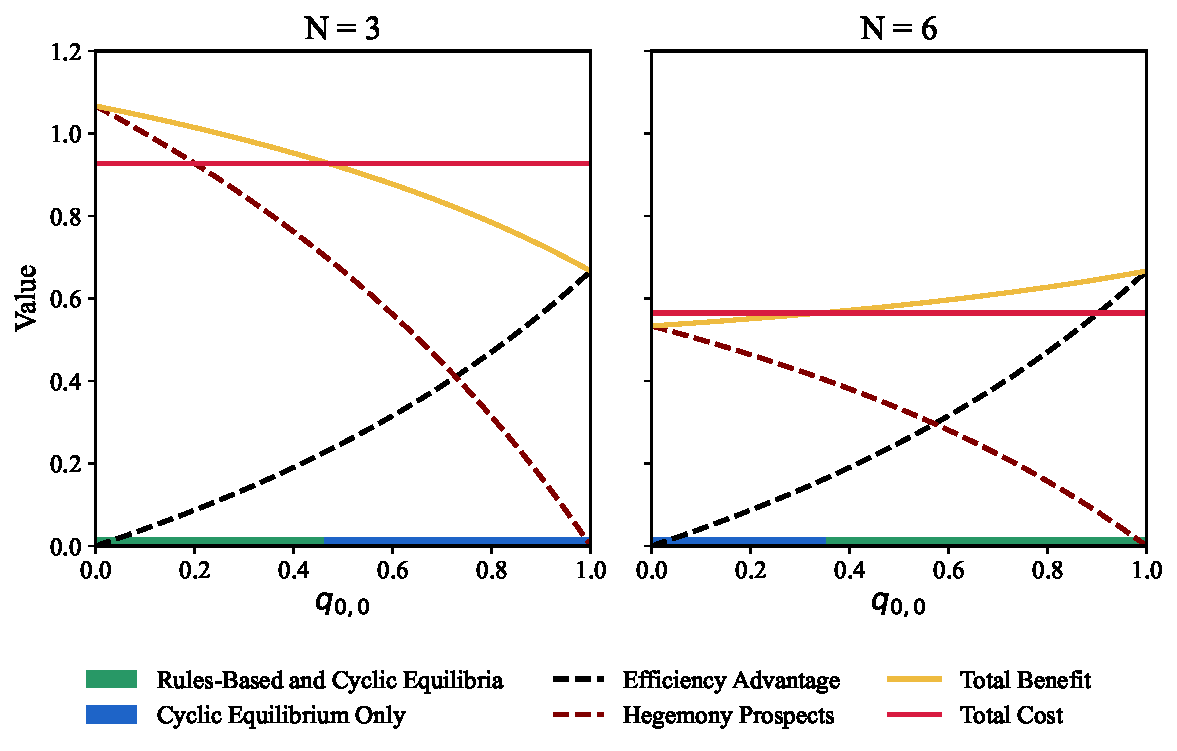
\includegraphics[width=0.85\linewidth]{fig_2_1_multipolar_persistence.pdf}
\caption{Figure 2.1, Multipolar fragmentation and persistence effects on rules-based equilibria}
\label{fig:21}
\begin{minipage}{0.9\linewidth}
\vspace{4pt}
\footnotesize\raggedright
\textit{Notes:} \code{python/persistence.py} ($c = 8$, $\delta = 0.4$,
$N \in \{3, 6\}$) $\rightarrow$ \code{persistence.pdf}.
\end{minipage}
\end{figure}
